\documentclass[a4paper]{article}
\usepackage{graphicx} % Untuk menambahkan gambar
\usepackage{geometry} % Untuk mengatur margin
\usepackage{float}    % Untuk mengontrol posisi gambar

% Mengatur ukuran kertas dan margin
\geometry{
    a4paper,
    left=2cm,
    right=2cm,
    top=3cm,
    bottom=2cm
}

\title{Judul Dokumen Anda}
\author{Nama Anda} 
\date{\today}
\begin{document}

\section*{Edgrant Henderson Suryajaya}
\textbf{\huge{Mata Kuliah - K4}} \\
\vspace{\baselineskip}

\begin{figure}[htp]
    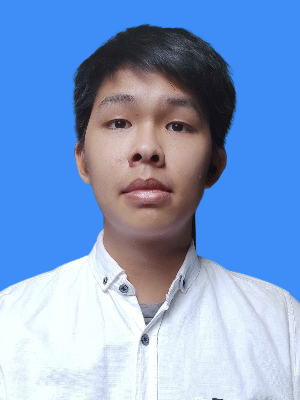
\includegraphics[width=0.25\linewidth]{pasfoto.png}
    \label{fig:enter-label}
\end{figure}

\vspace{2em}

\noindent \textbf{Nama Lengkap} adalah Edgrant Henderson Suryajaya.

\section*{Arti dan Makna Nama}
\begin{itemize}
    \item \textbf{\textit{Ed}}: nama ini berasal dari bahasa ingris kuno \textit{ēad}, berarti ``Keberuntungan''.
    
    \item \textbf{\textit{Grant}}: nama ini berasal dari bahasa Inggris, berarti ``besar''. Jika digabung dengan nama sebelumnya, artinya menjadi ``Keberuntungan Besar''. Orang tua saya memberikan nama ini dengan harapan agar saya dapat meraih kesuksesan yang besar dalam hidup.

    \item \textbf{\textit{Henderson}}: Henderson berarti anak dari Hendry, yaitu ayah saya. Nama ini diberikan sebagai bentuk penghormatan kepada ayah saya.
    
    \item \textbf{\textit{Suryajaya}}: Suryajaya merupakan marga saya.
\end{itemize}

\section*{Harapan Pemberi Nama}
Orang tua saya memberikan nama ini dengan tujuan agar saya dapat:
\begin{enumerate}
    \item Meraih kesuksesan yang besar dalam hidup.
    \item Menjadi anak yang berbakti kepada orang tua.
\end{enumerate}


\section*{Kontribusi Bagi Kesejahteraan Pribadi dan Lingkungan serta Hubungannya dengan Nama}
Saya percaya bahwa kesejahteraan pribadi tidak terlepas dari kesejahteraan lingkungan sekitar. Nama yang diberi setiap orang memiliki makna dan harapan tersendiri. Dengan memahami makna nama, seseorang dapat memahami harapan orang tua. Dengan demikian, seseorang dapat berusaha untuk meraih harapan tersebut dan memberikan kontribusi bagi kesejahteraan pribadi dan lingkungan sekitar. Dengan nama yang memiliki makna ``Keberuntungan Besar'', saya telath kontribusi bagi keselamatan dan kesejahteraan pribadi serta lingkungan sekitar dengan
\begin{itemize}
    \item Menjadi pribadi yang berusaha meraih kesuksesan yang besar dalam hidup. Dengan demikian, saya dapat memberikan kontribusi bagi kesejahteraan pribadi dan lingkungan sekitar.
    \item Selalu mencoba menjaga keamanan dan kesejahteraan sekitar dengan berperilaku baik dan bertanggung jawab.
\end{itemize}
\end{document}